\section{Towards a common language for computational dynamics}
Three of the most successful branches of scientific discourse all agree on the shape of a model adequate for expressing and effecting computation. Physics, computer science, and mathematics all use the same standard shape. A model adequate for computation comes with an algebra of states and “laws of motion.”

One paradigmatic example from physics is Hilbert spaces and the Schroedinger equation. In computer science and mathematics the algebra of states is further broken down into a monad (the free algebra of states) and an algebra of the monad recorded as some equations on the free algebra.

Computer science represents laws of motion, aka state transitions, as rewrite rules exploiting the structure of states to determine transitions to new states. Mainstream mathematics is a more recognizable generalization of physics, coding state transitions, aka behavior, via morphisms (including automorphisms) between state spaces.

But all three agree to a high degree of specificity on what ingredients go into a formal presentation adequate for effecting computation.

\subsection{Examples from computer science}
Since Milner's seminal Functions as processes paper, the gold standard for a presentation of an operational semantics is to present the algebra of states via a grammar (a monad) and a structural congruence (an algebra of the monad), and the rewrite rules in Plotkin-style SOS format.

\subsubsection{$\lambda$-calculus}

\paragraph{Algebra of States}
\begin{eqnarray*}
  Term[V] & \bc & V \\
  & \;\bm\; & \lambda V.Term[V] \\
  & \;\bm\; & \mathsf{(} Term[V] \; Term[V] \mathsf{)}
\end{eqnarray*}

The structural congruence is the usual $\alpha$-equivalence, namely that $\lambda x.M \scong \lambda y.(M\{y / x\})$ when $y$ not free in $M$.

It is evident that $Term[V]$ is a monad and imposing $\alpha$-equivalence gives an algebra of the monad.

\paragraph{Transitions}
The rewrite rule is the well know $\beta$-reduction.
\begin{mathpar}
  \inferrule* [lab=Beta]{}{((\lambda x.M)N) \to M\{N / x\}}
\end{mathpar}

\subsubsection{$\pi$-calculus}

\paragraph{Algebra of States}
\begin{eqnarray*}
  Term[N] & \bc & \mathsf{0} \\
  & \;\bm\; & \mathsf{for}\mathsf{(}N \leftarrow N\mathsf{)}Term[N] \\
  & \;\bm\; & N\mathsf{!}\mathsf{(}N\mathsf{)} \\
  & \;\bm\; & \mathsf{(}\mathsf{new}\; N\mathsf{)}Term[N] \\
  & \;\bm\; & Term[N] \; \mathsf{|}\; Term[N] \\
  & \;\bm\; & \mathsf{!}Term[N]
\end{eqnarray*}

The structural congruence is the smallest equivalence relation including $\alpha$-equivalence making $(Term[N],\;\mathsf{|}\;,\mathsf{0})$ a commutative monoid, and respecting

\begin{eqnarray*}
  \mathsf{(}\mathsf{new}\; x\mathsf{)}\mathsf{(}\mathsf{new}\; x\mathsf{)}P & \scong & \mathsf{(}\mathsf{new}\; x\mathsf{)}P \\
  \mathsf{(}\mathsf{new}\; x\mathsf{)}\mathsf{(}\mathsf{new}\; y\mathsf{)}P & \scong & \mathsf{(}\mathsf{new}\; y\mathsf{)}\mathsf{(}\mathsf{new}\; x\mathsf{)}P \\
  (\mathsf{(}\mathsf{new}\; x\mathsf{)}P)\mathsf{|}Q & \scong & \mathsf{(}\mathsf{new}\; x\mathsf{)}(P\mathsf{|}Q), x \notin \freenames{Q}
\end{eqnarray*}

Again, it is evident that $Term[N]$ is a monad and imposing the structural congruence gives an algebra of the monad.

\paragraph{Transitions}
The rewrite rules divide into a core rule, and when rewrites apply in
context.
\begin{mathpar}
  \inferrule* [lab=COMM]{}{\mathsf{for}\mathsf{(}y \leftarrow x\mathsf{)}P \mathsf{|} x\mathsf{!}\mathsf{(}z\mathsf{)} \to P\{ z / y \}} \\
  \and  
  \inferrule* [lab=PAR]{P \to P'}{P\mathsf{|}Q \to P'\mathsf{|}Q}
  \and
  \inferrule* [lab=STRUCT]{P \scong P' \to Q' \scong Q}{P \to Q}
\end{mathpar}

\subsubsection{rho-calculus}

\paragraph{Algebra of States}
Note that the rho-calculus is different from the $\lambda$-calculus and the $\pi$-calculus because it is \emph{not} dependent on a type of variables or names. However, it does give us the opportunity to expose how ground types, such as Booleans, numeric and string operations are imported into the calculus. The calculus does depend on the notion of a $0$ process. In fact, this could be any builtin functionality. The language rholang, derived from the rho-calculus, imports all literals as \emph{processes}. Note that this is in the spirit of the $\lambda$-calculus and languages derived from it: Booleans, numbers, and strings are terms, on the level with $\lambda$ terms.

So, the parameter to the monad for the rho-calculus takes the collection of builtin processes. Naturally, for all builtin processes other than $0$ there have to be reduction rules. For brevity, we take $Z = \{0\}$.
\begin{mathpar}
\inferrule* [lab=process] {} {Term[Z] \bc Z \;\bm\; \mathsf{for}(
  Name[Z] \leftarrow Name[Z] )Term[Z] \;\bm\; Name[Z]\mathsf{!}(Term[Z]) 
  \\ \and \;\bm\; \mathsf{*}Name[Z] \;\bm\; Term[Z]\mathsf{|}Term[Z] } \\
\and \inferrule* [lab=name] {}
     {Name[Z] \bc \mathsf{@}Term[Z] }
\end{mathpar}

The structural congruence is the smallest equivalence relation including $\alpha$-equivalence making $(P,\;\mathsf{|}\;,\mathsf{0})$ a commutative monoid.

Again, it is evident that $Term[Z]$ is a monad and imposing the structural congruence gives an algebra of the monad.

\paragraph{Transitions}
The rewrite rules divide into a core rule, and when rewrites apply in
context.
\begin{mathpar}
  \inferrule* [lab=COMM] {x_{t} \;\nameeq\; x_{s}} {\mathsf{for}(y \leftarrow x_{t} )P \;\mathsf{|}\; x_{s}!(Q)
  \red P\substn{\quotep{Q}}{y}} \\
  \and
  \inferrule* [lab=PAR]{P \red P'}{P\mathsf{|}Q \red P'\mathsf{|}Q}
  \and
  \inferrule* [lab=STRUCT]{{P \;\scong\; P'} \andalso {P' \red Q'} \andalso {Q' \;\scong\; Q}}{P \red Q}
\end{mathpar}

\pagebreak
\subsubsection{The JVM}

While its complexity far exceeds the presentations above, the JVM specification respects this same shape. Here is an example from the specification of what the operation aaload does.

\begin{figure}[h!]
  \scalebox{0.75}{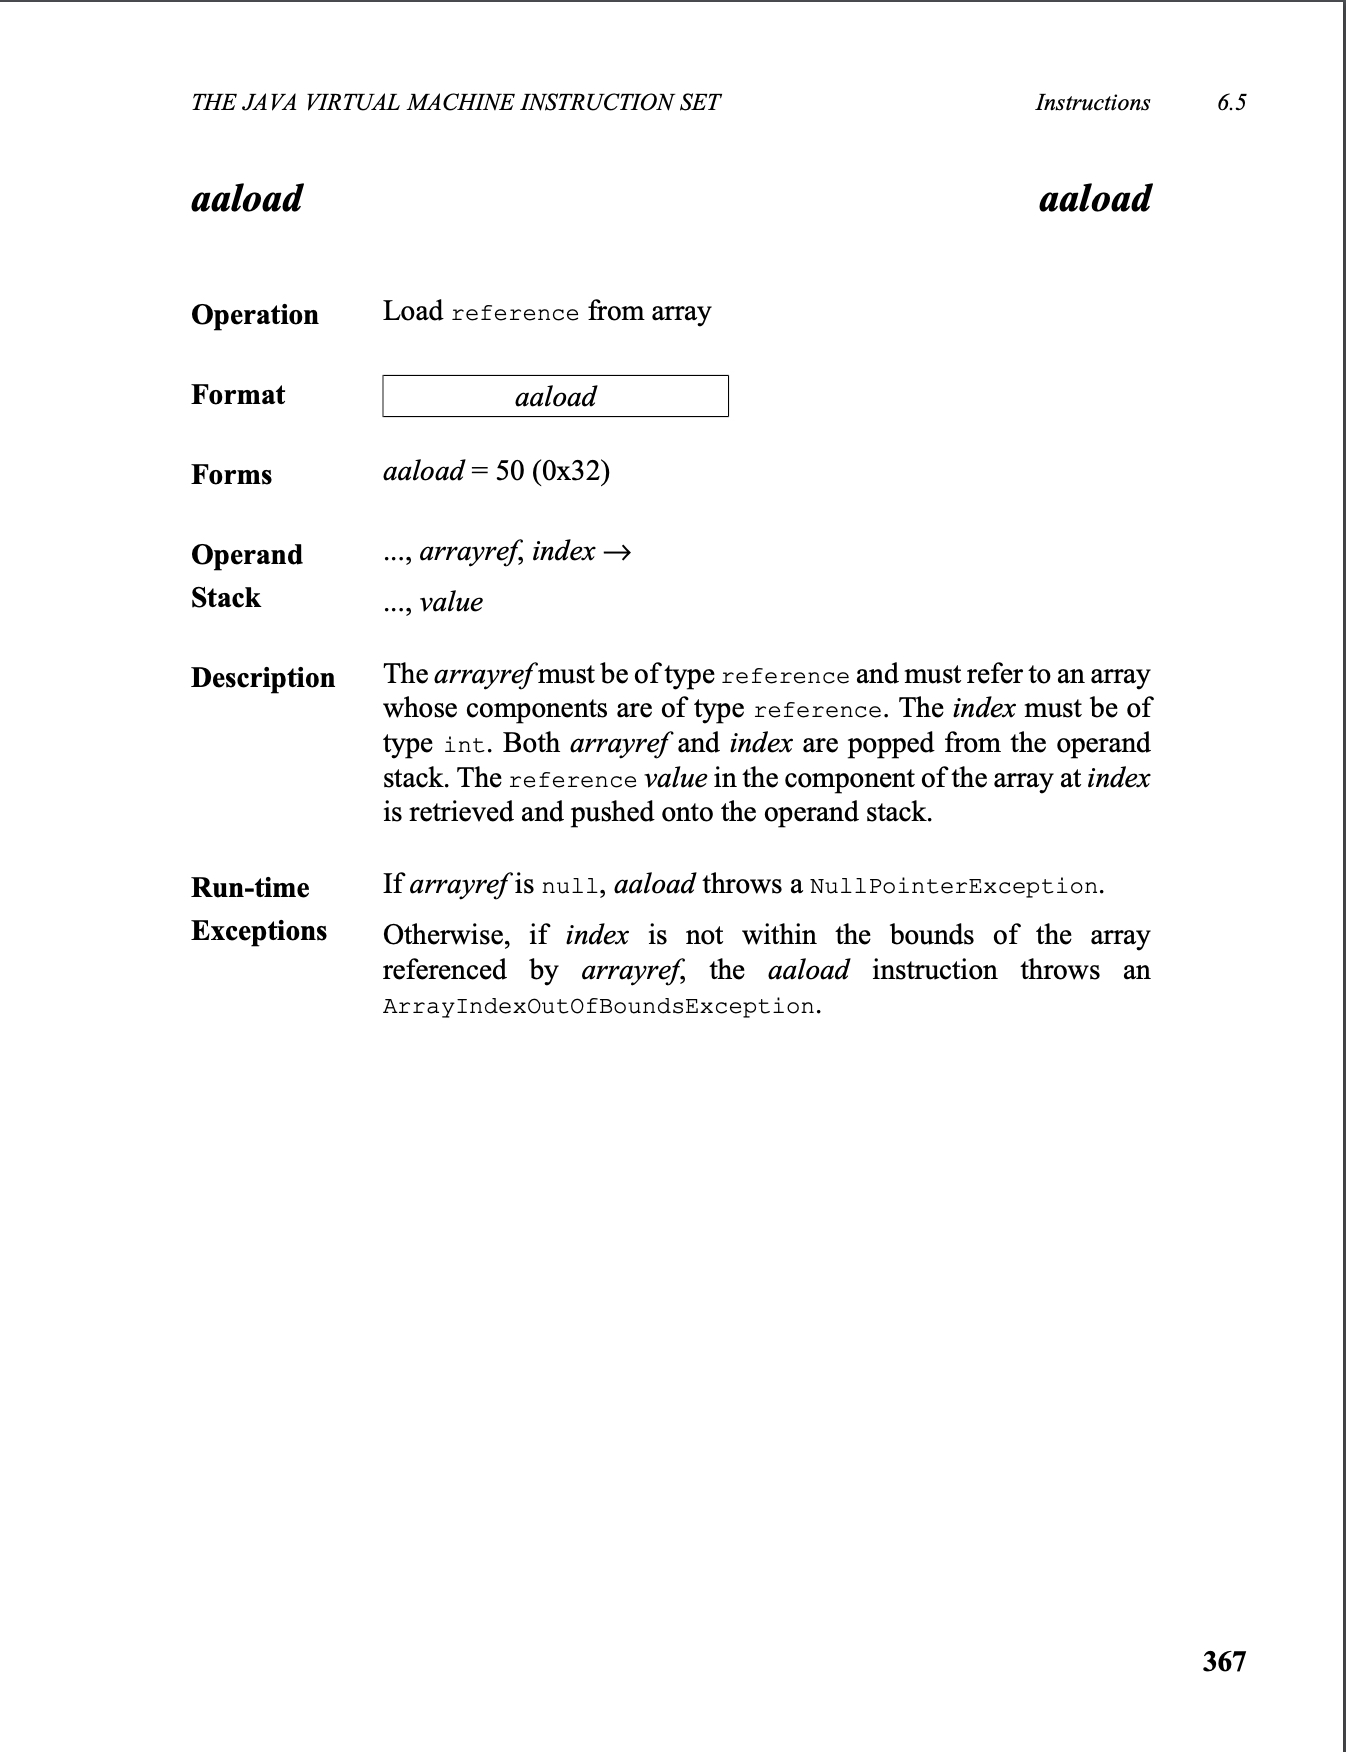
\includegraphics[width=\linewidth]{JVMSpecAALOAD.jpg}}
  \caption{AALOAD instruction specification}
  \label{fig:AALOADSpec}
\end{figure}

\paragraph{WYSIWYG semantics}One important point about the JVM versus the previous three
examples. The first three examples are examples of WYSIWYG operational
semantics in the sense that the states \emph{are} the terms of the
calculi. In the case of the JVM the terms in the language are only
part of the state, which includes the stack, the heap, and several
registers. WYSIWYG models make static analysis dramatically
simpler. Specifically, an analyzer only has to look at terms in the
language.
